\chapter{SpaceRL: Our Knowledge graph reasoning proposal.}\label{chap:SpaceRL}

\chapterQuote{\hfill\textit{``Reason has always existed, but not always in a reasonable form.''}}{--- Karl Marx}

\chapterAbstract{W}{hen presented with the challenge of completing a given knowledge graph we must aim to offer the most complete answer possible, a reasoned answer that complements the inference achieved, that responds to the question of why the knowledge presented must be incorporated back into the graph. In this chapter, we introduce SpaceRL our knowledge graphs reasoning proposal. This chapter is structured as follows: Section~\ref{sec:spacerl-intro} introduces the proposal , Section~\ref{sec:spacerl-formal_description} Formally introduces the problem to solve., Section~\ref{sec:spacerl-proposal} Presents the developments made in the work, Section~\ref{sec:spacerl-evaluation} Explains the methodology followed to evaluate the methods and displays the results obtained by them, Section~\ref{sec:spacerl-limitations} touches on the limitations of the method, Lastly, Section~\ref{sec:spacerl-summary} summarizes the work.}

\section{Introduction}\label{sec:spacerl-intro}
This chapter introduces SpaceRL-KG our KG reasoning proposal using Reinforcement Learning with embedding-based rewards.

\begin{figure}[htp]
    \centering
    \includesvg[inkscapelatex=false, width=\textwidth]{fig/SpaceRL-KG/Example_KG}
    \caption{An example Knowledge Graph with possible new relations as dotted lines.}
    \label{fig:kg-example}
\end{figure}

To apply RL to Knowledge Graph Completion, we train a Reinforcement Learning agent that learns how to navigate through the graph and generate new reasoned paths that can be applied back as new triples.

Using the graph from Figure~\ref{fig:kg-example} as an example we will overview how the agent would infer the new knowledge (``Alexandra Grant'', ``speaks'', ``English'').

The agent would start at the subject node (``Alexandra Grant'') and decide what edges should be traversed to reach the target node (``English''), these edges are represented as triples ($node_0$, $relation$, $node_1$) indicating directionality.
In this case, the agent could deduce that Alexandra Grant speaks English by navigating through several paths, such as:

\begin{center}
(Alexandra Grant, ¬is\_partner, Keanu Reeves) $\rightarrow$ \\
(Keanu Reeves, speaks, English) 
\end{center}

\begin{center}
(Alexandra Grant, ¬is\_partner, Keanu Reeves) $\rightarrow$ \\
(Keanu Reeves, lives\_in, Toronto) $\rightarrow$ \\
(Toronto, official\_lang, English)
\end{center}

The relational paths are then registered as possible answers to the query (``Alexandra Grant'', ``speaks'', ``?'') where the sum of the relations of the path would equal the missing target relation ``speaks'', in this case, the relational paths are the following.

\begin{center}
    ($e_0$, ¬is\_partner, $e_1$, lives\_in, $e_2$, official\_lang, $e_q$) = ($e_0$, speaks, $e_q$)\\
    ($e_0$, ¬is\_partner, $e_1$, speaks, $e_q$) = ($e_0$, speaks, $e_q$)
\end{center}

In this example it is confirmed by two separate paths that Alexandra Grant speaks English, the more this relation chain appears in the graph, the more trustworthy it becomes. These reasoned paths can be directly translated into new graph triples or presented to users for human-in-the-loop relation classification operations.

The application of RL to KG reasoning tasks requires that the entities and edges of the graph be transformed into numerical vectors that can be provided to the agents as a representation of the state and its available actions at every step.

SpaceRL-KG focuses on an improved set of rewards and the application of novel algorithms to these processes. The evaluation of our technique is performed by applying it to several widely accepted Knowledge Graphs and shows that our novel reward functions significantly improve performance when compared to more traditional ones, especially when node embeddings are used.
Throughout this chapter, we will expand on the running example in Section~\ref{sec:spacerl-intro}.

\section{Formal Description}\label{sec:spacerl-formal_description}

\todo{ se ha separado cada parte de la estructura formal del problema y solucion en los diferentes apartados y este se ha reservado tan solo para la descripcion formal del problema.}

Knowledge graphs $\mathcal{K}$ are formally represented as a set of entities $\mathcal{E}$ and relations $ \mathcal{R}$ Where ($s, r, o$) denotes a triple in the graph, representing a fact that connects entity $s$ to $o$ via a relation $r$ formally described by equation \ref{eq:formalKG}. 

\begin{equation}
\label{eq:formalKG}
\mathcal{K} = \{ (s, r, o) ~|~ s, o \in \mathcal{E}, r \in \mathcal{R} \}
\end{equation}

We assume that, due to its nature, \( \mathcal{K} \) is inherently incomplete concerning the information that we know to be true in the real world.

In order to find missing edges in these Knowledge Graphs we perform a multi-hop approach where the input is a query represented by a source node and a relation $(e_0,r_q)$ and the output is a path of predetermined length $n$ that should reach the answer node of the missing edge, $e_a$. This path can be represented as:

\begin{equation}
\label{eq:formalPath}
p_k(e_0,e_k) =  \Bigl\{ e_0 \xrightarrow[]{r_0} e_1 \xrightarrow[]{r_1} ... \xrightarrow[]{r_n} e_n \Bigl\}
\end{equation}

And it is considered to be correct if $e_n = e_a$, where $e_n$ is the node in step n, the last step in the path. We could then infer a new relation ($e_0\xrightarrow[]{r_q}e_n$).

\section{Our proposal}\label{sec:spacerl-proposal}
As we have already seen in previous sections SpaceRL-KG focuses on acquiring reasoned knowledge in the form of paths in order to determine if a particular relation should exist between two nodes of the graph.
It does so by training intelligent agents by way of applying novel reward functions and algorithms in a Reinforcement Learning setup, where the Knowledge Graph acts as the environment and each node as the state.

To obtain these paths the graph nodes and relations must be encoded as numerical vectors representing their position in a N-dimensional space. 
These numerical vectors are then combined in a way where they represent the current state, a possible action and the context of the episode. this information is then fed to a Neural Network which represents the agent policy, responsible for selecting the best-estimated action for every episode step.

This is done by evaluating every possible action for every step of the path and then stochastically selecting one based on the policy scores provided, the agent is then rewarded based on several metrics and updated after every episode.

\subsection{Embedding representations}\label{sec:spacerl-embeddings}

\subsection{Reinforcement Learning implementation}\label{sec:spacerl-rlimplementation}

Any application of Reinforcement Learning to knowledge graphs can be formalized as a Markov decision process, assuming that several conditions are met beforehand. By adding inverse edges to the graph, path connectivity is guaranteed: if the edge $(e_i,r,e_{i+1})$ exists in the graph, so does $(e_{i+1},\neg r,e_i)$, where $\neg r$ denotes the inverse relation to $r$. During the training of the model, we remove the edges that are used to create queries in order to simulate the absence of their direct answers and prevent the agent from taking the direct path to the target entity. Self-loop edges are also added beforehand; these represent the NO-OP action, which entails that an agent chooses to stay in the current node, which is desirable if the answer node is reached before advancing $n$ steps. This introduces a new edge $(e_i,r_{NO-OP},e_i)$ per entity. Staying in the current node might cause local minimum stagnation, which is undesired behavior and should be accounted for by the reward function.

We can define the following elements typical of a Markov process that, in turn, make up the agent and the environment:

\textbf{State:} The state $S_t$ at a certain step $t \in 0..n$ is defined as the combination of the query $(e_0, r_q)$, the destination node $e_n$ and the current location $e_t$. We can formally define the state as follows: $S_t \in \mathcal{S} ~\|~ S_t = (e_t, e_0, r_q, e_a)$ where $\mathcal{S}$ is the set of all possible states.

\textbf{Observations:} The environment is not fully observed by the agent: in any given state $S_t$ the agent is only aware of its current location $e_t$ and the query $(e_0,r_q)$. Formally, $O_t \in \mathcal{O} ~\|~ O_t = (e_t, e_0, r_q)$ where $\mathcal{O}$ is the set of all possible agent observations.

\textbf{Actions:} The set of all actions an agent can take in a given state $t$ depends on the current location, $e_t$. Since the location represents a node in the graph with one or more connected edges, these edges are the possible actions of the agent. Formally we describe the action space for a given location $e_t$ with 

\begin{equation}
\label{eq:ActionSpace}
\mathcal{A}_t  = \Bigl\{ (e_t,r_i,e_i)  \|  S_t = (e_t,e_0,r,e_a) , r_i \in   \mathcal{R}_i ,  e_i \in   \mathcal{E}_i  \Bigl\}
\end{equation}


where $\mathcal{R}_i,\mathcal{E}_i$ denote the subset of relations and entities from the edges connected to $e_{t}$ respectively. In simpler terms the agent can select any of the outgoing edges, being aware of the node it reaches.

\textbf{Transition:} The transition refers to how the environment evolves after the agent takes an action. In this case this happens in a deterministic manner as previously mentioned, updating the set of available actions to those of the new node that the agent reached through the selected action. The new state remains the same except for the location, which becomes the node reached by the chosen action. Formally, this is represented by a transition function involving the state and the action space such as $\mathcal{P}( \mathcal{S,A} ) = \mathcal{P}(e_t ,(e_0,r_q), \mathcal{A} _t))$, where $(e_0,r_q)$ denotes the query, $e_t$ the current location, and  $\mathcal{A}_t$ the action space for that location.

\textbf{Rewards:} For the computation of the reward, we have defined several components that can be toggled or applied with lesser or greater weights:

\begin{itemize}
    \item \textbf{Terminal}: a binary \{1,0\} reward that is given to the agent whenever it is located in the answer node $e_a$. If triggered, this reward overrides all other reward components.
    \item \textbf{Distance}: a reward component based on the distance to the answer node (length of the shortest path). Shorter distances lead to higher rewards.
    \item \textbf{Embedding}: a reward component based on several properties of the embedding representation of nodes and relations, representing semantic similarity. Higher semantic similarity leads to higher rewards.
    \item \textbf{Shaped}: a variant of the terminal reward function that replaces the 0 score associated with not reaching the target node with an embedding-based score computed from the starting node, the relation representing the question, and the reached node. Note that this reward does not compare the reached node with the target one, but uses traditional embedding-based score as a fallback function.
    \item \textbf{NO-OP}: a negative reward that aims to discourage the use of the no-op action outside the answer node. This reward overrides all other reward components, and cannot be triggered in the same step as the terminal reward.
\end{itemize}

Detailed information regarding the distance and embedding rewards can be found in Section \ref{sec:spacerl-rewards} Shaped reward were implemented as seen in approaches \cite{cui2023incorporating, lin2018multi} for comparison purposes; they use embeddings, however, they do so in a  different manner, only using them as an anticipation or guiding factor and relying in terminal rewards.

\begin{figure*}[!h]
    \makebox[\textwidth][c]{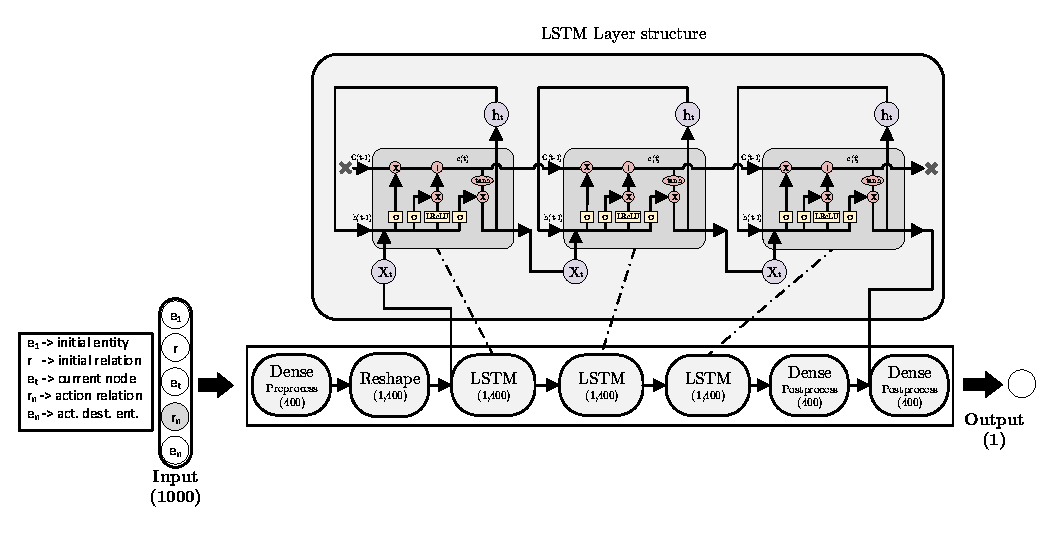
\includegraphics[width=1\textwidth]{fig/SpaceRL-KG/Agent_Policy.eps}}
    \caption{Policy architecture.}
    \label{fig:policy}
\end{figure*}

\subsection{Policy Network}
\label{sec:spacerl-policy}

The policy used to determine which action will be taken at each step is based on the neural network architecture described in Figure~\ref{fig:policy}. The network receives state information in the form of the query $(e_0,r_q)$, the current location node $e_t$ as well as the action which is being evaluated $(r_{t+1}, e_{t+1})$. These actions are all the possible relations connected to the current node $e_t$. It is necessary to evaluate each action individually since the number of edges connected to a node is variable.

For the neural network to receive this information, it is encoded using translation embedding representations for each of the entities and relations so that  $\textbf{r} \in \mathbb{R}$, $\textbf{e} \in \mathbb{E}$ where $\mathbb{R}$ and $\mathbb{E}$ are the vectorial spaces containing all possible representations in the graph. The chosen size for these embedded representations was $200$ as it is a common in literature for these set of knowledge graphs and embedding combinations, making the networks input size $1000$ units.

The embedding vectors are concatenated and fed to the network as $[e_q,r_q,$ \\$e_t,r_{t+1},e_{t+1}]$. The input is passed on to a densely connected layer for pre-processing, whose output is connected to a multi-layered Long short-term memory (LSTM) \cite{hochreiter1997long} block with 3 layers. The result is post-processed with 2 more dense layers that produce a numerical answer representing the quality of the selected action. The final output is produced by a sigmoid function(~\ref{eq:sigmoid}) that produces a [0,1] output that is adequate for an action evaluator.

\begin{equation}
\label{eq:sigmoid}
    \sigma(z) = \frac{1} {1 + e^{-z}}
\end{equation}

The activation function in intermediate layers was chosen to be leaky ReLU to avoid gradient explosion \cite{bengio1994learning}, which is common in deep neural approaches. Batch normalization is applied to the embedding representations, and ADAM \cite{kingma2014adam} is used as optimizer. 

The historical values $h_t = (e_0,r_1,e1,...,r_n,e_n)$ can be formally defined by equation(~\ref{eq:ht}) for the hidden state layer of LSTMs at instant t.

\begin{equation}
\label{eq:ht}
    h_t = LSTM_{enc}((r_t,e_t), h_{t-1})
\end{equation}

Finally the policy network can be formalized as:

\begin{equation}
\label{eq:pn}
\begin{split}
    & \pi_s(a_t|s_t) = \sigma(\mathcal{A}_t \text{x} \mathcal{S}_t [W_6;W_5]ReLU([W_4-W_2]\text{x}[e_t;r_t;h_t]ReLU(W_1[e_t;r_t])))
\end{split}
\end{equation}


\subsection{Embedding \& Distance rewards}
\label{sec:spacerl-rewards}

\begin{algorithm}[!h]
\caption{Embedding-based reward calculation}
\label{alg:embeddings}
\KwIn{\\
\texttt{// Previous location values.}\\
$PrevDot$, $PrevEucDist$, $PrevCosSim$:\textless Float\textgreater\\
\texttt{// Embedding of the current node}\\
$e_t$: List\textless Float\textgreater\\
\texttt{// Embedding of the goal node}\\
$e_a$: List\textless Float\textgreater\\
}
\KwOut{$reward$: Float}

$dot \gets e_t \cdot e_a$ // ``·'' is the dot product operator. \\ 
$euc\_dist \gets norm(e_t - e_a)$\\
$cos\_sim \gets dot ~/~ (norm(e_t) \times norm(e_a))$\\
$reward \gets 0.0$\\

\uIf{$PrevDot > dot$}{
    $reward \mathrel{+}= \frac{1}{3}$
}\ElseIf{$PrevDot = dot$}{
   $reward \mathrel{+}= \frac{1}{6}$
}

\uIf{$PrevEucDist > euc\_dist$}{
    $reward \mathrel{+}= \frac{1}{3}$
}\ElseIf{$PrevEucDist = euc\_dist$}{
    $reward \mathrel{+}= \frac{1}{6}$
}

\uIf{$PrevCosSim > cos\_sim$}{
    $reward \mathrel{+}= \frac{1}{3}$
}\ElseIf{$PrevCosSim = cos\_sim$}{
    $reward \mathrel{+}= \frac{1}{6}$
}

\Return $reward$
\end{algorithm}

These reward functions act on a step by step basis, that is, they are calculated at every step independently of whether or not the answer node was reached. The embedding reward is based on the property of translational embeddings according to which the combination of an entity and a connecting relation results in a very similar vector to the target entity. We leverage this information to define a new reward component, as shown in Algorithm~\ref{alg:embeddings}. This function intends to reward the semantic similarity between the reached node and the answer node. This is done by measuring the distance between their embedding representations using several distance functions and checking whether such distance has decreased with respect to the former step.

\newcommand{\pluseq}{\mathrel{+}=}

\begin{algorithm}[!h]
    \caption{Distance reward calculation}
    \label{alg:distance}
    \KwIn{\\
    \texttt{// Current distance to goal node}\\
    $d_t$: Integer\\
    \texttt{// Previous distance to goal node}\\
    $d^{-1t}$: Integer\\
    }
    \KwOut{$reward$: Float}

    $reward \gets 0.0$

    \uIf{$d_t < d^{-1t}$}{
        $reward \gets 1$
    }\ElseIf{$d_t = d^{-1t}$}{
        $reward \gets \frac{1}{3}$
    }

    \Return $reward$
\end{algorithm}


The distance reward is computed according to the length of the shortest path from the currently explored node $e_t$ to the answer node $e_a$. The distance is calculated by performing a tree exploration of the graph, which is an expensive operation. This is why we opted for caching computed distances in order to share these data between training episodes. The calculated distance $d$ is then compared against the previously computed distance $d^{-1}$ at $e_{t-1}$ to check if the chosen action got the agent closer to the end node. This way, the agent is rewarded by moving faster towards the answer node, which results in shorter paths without the need of limiting their length excessively by reducing $n$.
% Calculating the distance reward implies that all paths of length $n$ could be known, however this does not make every path valid. Applying this method to KGC would simply fill the graph with new triples which in most cases wouldn't be new facts and would only dilute the existing ones.
The distance reward function is shown in detail in Algorithm~\ref{alg:distance}.


\subsection{Reinforcement Learning algorithms}
\label{sec:spacerl-RLalgorithms}

% As it can be seen in Table~\ref{tab:SoTA_approaches}, all previous completion approaches use the REINFORCE algorithm as their parametrization method to maximize expected rewards. This algorithm is optimized for terminal rewards or similar ones which are only triggered at the end of an episode, when the obtained rewards are then backpropagated to the former steps in the episode. Formally, the REINFORCE algorithm is described as follows:

\todo{re-wrie this without making references to the table of SoTa approaches.}

\begin{equation}
\label{eq:reinforce}
    \Delta_{\theta}\mathcal{J}(\theta) =\Delta_{\theta}log\pi_{\theta}(s,a)\mathcal{G}(s,a) 
\end{equation}

where $\mathcal{J}$ can be any loss function and $\mathcal{G}$ is the propagated reward in the action state pair (a,s).

This approach, however, suffers from some known shortcomings:
\begin{itemize}
    \item {Since the agent takes several actions during the episode, specially if several episodes take place during the same learning loop for faster training times, the variance of the method increases (that is, a single reward is used to influence many different actions), and it becomes less likely to assign proper credit to the actually useful actions. Because of this, it takes more time for the gradients of the agent to converge, increasing the training time needed to stabilize the value of the loss function.}
    \item {REINFORCE only produces training data when episodes conclude, meaning that it is not possible to train an agent with a single, longer episode. This, however, has no effect in our context since all episodes are limited to a number of steps N.}
    \item {REINFORCE is very sensitive to hyperparameters, making it crucial to tune them for each approach, as seen in MINERVA\cite{das2017go}, here a hyperparameters table is specified for the performed tasks.}
\end{itemize}

To overcome REINFORCE's limitations, several other paradigms have been developed. We have identified as particularly promising the Proximal Policy Optimization (PPO) \cite{schulman2017proximal} and Actor-Critic \cite{castro2010convergent} approaches, in particular, the soft variant \cite{haarnoja2018soft}. These algorithms mitigate the aforementioned problems.
Their combination benefits from the advantages typical of Temporal-Difference Learning \cite{sutton1988learning} by defining a critic: a neural network tasked with predicting the value of the long-term reward associated to an action-state pair $(a,s)$. This value is used in a similar fashion to how Q-learning \cite{watkins1992q} uses the Q-value in its learning process. The values provided by the critic $\mathcal{C}(s,a)$ replace $\mathcal{G}(s,a)$ in equation \ref{eq:reinforce}, which results in the following equation:

\begin{equation}
\label{eq:ActorCritic}
    \Delta_{\theta}\mathcal{J}(\theta) =\Delta_{\theta}log\pi_{\theta}(s,a)\mathcal{C}(s,a) 
\end{equation}

We then learn the equivalent Q-value through the aforementioned TD-learning techniques, formally described as:

\begin{equation}
\label{eq:TemporalDifference}
\begin{split}
    \mathcal{C}(s,a) \gets \mathcal{Q}(s,a) + \alpha(r(s,a) + max_{a+1} \gamma \mathcal{Q}(s^{-1},a^{-1}) - \mathcal{Q}(s,a))
\end{split}
\end{equation}

where $a+1$ denotes the possible action values in the next step, $\alpha$ and $\gamma$ are numerical hyperparameters, and $\mathcal{Q}(s,a)$ denotes the output given by the actor from the action value pair $(s,a)$.

This approach reduces the variance significantly as we can update the parameters in a step by step basis by using the Q-value-like method, ensuring faster convergence of the policy gradient and making it possible to run a non-episodic method.

\section{Evaluation}\label{sec:spacerl-evaluation}
In this section, we describe in detail the experiments we carried out to evaluate our contributions and their results. First, we introduce the datasets we use in our experiments. Then, we describe the experimental setup, that is, the techniques that are evaluated and under what conditions. Finally, we provide a discussion of the results obtained in our experiments.


\subsection{Experimental data}

We selected five benchmark datasets, which are often used in the literature, and which can help discern the strengths of the techniques under evaluation:

\begin{itemize}
    \item \textbf{COUNTRIES} \cite{bouchard2015approximate}, a small, low-connectivity dataset that contains relations between geographical regions and the countries inside them.
    
    \item \textbf{Unified Medical Language System (UMLS)} ~\cite{kok2007statistical}, a highly connected dataset that consists of biomedical data, with entities representing different diseases, bacteria, treatments and diagnoses.
    
    \item \textbf{FreeBase (FB15K-237)} \cite{toutanova2015representing}, a subset of the FreeBase Knowledge Graph in which inverse relations have been removed to avoid leakage from the training to testing validation splits.
    
    \item \textbf{Never Ending Language Learning (NELL-995)}\cite{xiong2017deeppath}, a particular version of the NELL dataset, built by web crawlers automatically by extracting triples from plain text from several sources.
    
    \item \textbf{WordNet (WN18RR)} \cite{miller1995wordnet}, a subset of WordNet in which originally many text triples are obtained by inverting triples from the training set. \cite{dettmers2018convolutional}
    This leads to these datasets being able to be completed by using simple ruling, by removing these inverse triples, WN18RR, avoids leakage of inverse relations into the testing split, thus making it necessary to have knowledge of the entire dataset.
\end{itemize}

Table~\ref{tab:datasets} contains a statistical summary of the aforementioned datasets.

\begin{table}[!h]
    \centering
    \resizebox{0.75\columnwidth}{!}{
        \begin{tabular}{l|ccccc}
            \toprule
            \multirow{2}{*}{Dataset} & \multicolumn{1}{c}{\multirow{2}{*}{\textbf{Entities}}} &\multicolumn{1}{c}{\multirow{2}{*}{\textbf{Relations}}} & \multirow{2}{*}{\textbf{Triples}} &\multicolumn{2}{l}{\hfill\textbf{Degree }} \\& \multicolumn{1}{c}{}& \multicolumn{1}{c}{}&& Mean& Median\\
            \bottomrule
            COUNTRIES& 272& 2& 1,159& 4.35& 4\\
            UMLS& 135& 49& 5,216& 38.63& 28\\
            FB15K-237& 14,505& 237& 272,115& 19.74& 14\\
            NELL-995& 75,492& 200& 154,213& 4.07& 1\\
            WN18RR& 40,945& 11& 86,835& 2.19& 2\\
            
            \bottomrule
        \end{tabular}
    }
    \caption{Datasets (Degree = degree of connectivity)}
    \label{tab:datasets}
\end{table}

% We evaluated our proposal using four KGs provided by the freely available AYNEC-DataGen~\cite{ayala2019aynec} tool: FB13-A, WN11-AR, WN18-AR and NELL-AR. These KGs are based on the well-known FB13, WN11 \cite{socher2013reasoning}, WN18~\cite{bordes2014constructing}, and a subset of NELL proposed in \cite{gardner2015}. However, they have been processed to remove reciprocal relations detected by AYNEC, i.e., relations $r$ and $r'$ such that, if $(s, r, t)$ exists, then $(t, r', s)$ also exists very frequently. Additionally, relations that amount to less than 5\% of the total number of triples in the graph have been removed.

\subsection{Experimental setup}
\begin{table}[!h]
\centering
\resizebox{0.85\columnwidth}{!}{
\begin{tabular}{>{}l|>{}c*{4}{>{}c}c}
\toprule
\multirow{2}{*}{\textbf{Metric}} & \multirow{2}{*}{\textbf{Embedding}} & \multicolumn{4}{c}{\textbf{Evaluation}} \\
\cmidrule(lr){3-6}
& & \textbf{COUNTRIES} & \textbf{UMLS} & \textbf{C-Normal} & \textbf{U-Normal} \\
\midrule
\multirow{4}{*}{HITS @1} & \textbf{TransE} & 0.819 & 0.298 & \textbf{1.000} & \textbf{1.000} \\
 & DistMult & 0.799 & 0.271 & 0.732 & 0.693 \\
 & ComplEx & 0.743 & 0.284 & 0.000 & 0.845 \\
 & TransR & 0.795 & 0.212 & 0.685 & 0.000 \\
\midrule
\multirow{4}{*}{HITS @3} & \textbf{TransE} & 0.996 & 0.656 & \textbf{1.000} & \textbf{1.000} \\
 & DistMult & 0.991 & 0.604 & 0.676 & 0.628 \\
 & ComplEx & 0.981 & 0.646 & 0.000 & 0.927 \\
 & TransR & 0.992 & 0.517 & 0.716 & 0.000 \\
\midrule
\multirow{4}{*}{HITS @5} & \textbf{TransE} & 1.000 & 0.832 & 0.000 & \textbf{1.000} \\
 & DistMult & 1.000 & 0.787 & 0.000 & 0.632 \\
 & ComplEx & 0.999 & 0.823 & 0.000 & 0.925 \\
 & TransR & 0.999 & 0.711 & \textbf{1.000} & 0.000 \\
\midrule
\multirow{4}{*}{HITS @10} & \textbf{TransE} & 1.000 & 0.973 & \textbf{1.000} & \textbf{1.000} \\
 & DistMult & 1.000 & 0.956 & 1.000 & 0.704 \\
 & ComplEx & 1.000 & 0.969 & 1.000 & 0.926 \\
 & TransR & 1.000 & 0.916 & 1.000 & 0.000 \\
\midrule
\multirow{4}{*}{MRR} & \textbf{TransE} & 0.904 & 0.520 & \textbf{1.000} & \textbf{1.000} \\
 & DistMult & 0.891 & 0.480 & 0.733 & 0.618 \\
 & ComplEx & 0.856 & 0.502 & 0.000 & 0.831 \\
 & TransR & 0.890 & 0.415 & 0.693 & 0.000 \\
 \bottomrule
\end{tabular}
}

\caption{Embedding comparison for the UMLS and COUNTRIES datasets}
\label{tab:embedding_comparison}
\end{table}

First, in order to limit our experimentation to a single type of embedding, we carried out a preliminary experimental study to determine which embeddings offered the best results. The results of this study are shown in Table ~\ref{tab:embedding_comparison}. It can be observed that TransE, despite its simplicity, leads to the best results in the COUNTRIES and UMLS datasets. Consequently, we use TransE for all of our experiments over the other three types that were tested (DistMult, ComplEx and TransR).

Previous to every training loop we make sure that the vectorial space of the embeddings is normalized, to avoid vanishing gradients or gradient explosions as previously mentioned. We set the hyperparameters to the following values: $\alpha=0.9$, $\gamma=0.99$, path exploration to a maximum of $5$, and hidden size of intermediate layers to $400$. These values were selected on an empirical basis, as to the best of our knowledge there is no way to systematically find the optimal ones for a given architecture.
For the Policy network, we set the kernel initializer to Glorot/Xavier \cite{glorot2010understanding} for general purpose or LeCun \cite{lecun2012efficient} for incompatible activation functions. We chose LReLU with a factor of $0.01$ as the activation for the intermediate layers to prevent gradient vanishing, which would lead to the Glorot activation being prevalent. We used L1 and L2 regularisation with L1 having a factor of $10^{-5}$ and L2 having $10^{-4}$. We selected RSMprop ~\cite{hinton2012neural}as an optimiser for the PPO network and Adam \cite{kingma2014adam} as default. The previous choices, were based on empirical testing performed by previous approaches \cite{jomaa2019hyp}.


We performed a preliminary evaluation of several techniques to select the most promising ones for further experimentation:

\begin{itemize}
    \item\textbf{Simple Terminal:} A non-retropropagated training with terminal reward and direct transmission of rewards, the simplest algorithm possible, that serves as a baseline.
    \item\textbf{Retropropagated Terminal:} A REINFORCE algorithm training with just a terminal reward. This strategy represents the current trends in the state-of-the-art.
    \item\textbf{Simple Embedding:} An embedding-based reward training with a simple algorithm.
    \item\textbf{Simple Distance:} A distance reward training with a simple algorithm.
    \item\textbf{Simple Combined:} A combinational reward training which uses both the embedding rewards (70\%) and the distance rewards (30\%), and a simple algorithm. The factor for each of the rewards is based on their previous performance when used individually.
    \item\textbf{Simple Distance (PPO):} A distance reward training with the PPO algorithm.
    \item\textbf{Simple Embedding (PPO):} An embedding reward training with the PPO algorithm.
\end{itemize}

\begin{figure*}[!h]
    \centering
    \includesvg[inkscapelatex=false, width=\textwidth]{fig/SpaceRL-KG/graphs/countries_trans_e.svg}
    \caption{comparison of metrics and techniques employed}
    \label{fig:metricsbarchart}
\end{figure*}

We generate a test and a training set from the triples in the dataset by following a 1-to-7 rotary rule, where $7$/$8$ of the total set would be selected at random and the remainder $1$/$8$ would be used as the test set. We evaluate the quality of the generated model by using two widely accepted performance measures: Mean Reciprocal Rank (MRR) of all correct entities, which is calculated as the mean of $1/rank_{e}$, with $rank_{e}$ being the ranking position of the target entity, and Hits@N, which is the percentage of cases in which $rank_{e}$ is above N. 

% \begin{table*}[!h]
    
% \resizebox{\columnwidth}{!}{
%     \begin{tabular}{l|ccccccc}
%         \hline
%         \textbf{Algorithm} & \multicolumn{5}{|c|}{\textbf{Base}} & \multicolumn{2}{|c}{\textbf{PPO}} \\
%         \hline
%         \textbf{Rewards} $\rightarrow$ & \multicolumn{1}{r}{\textbf{Retroprop}} & \multicolumn{6}{|c}{\textbf{Simple}} \\
%         \hline
%         \textbf{Metrics} $\downarrow$ & Terminal & Terminal & Embedding & Distance & Combined & Distance & Embedding \\
%         \hline
%         hits@1 & 0.568 & 0.355 & 0.758 & 0.682 & 0.592 & 0.792 & 0.830 \\
%         hits@3 & 0.912 & 0.732 & 0.982 & 0.974 & 0.86 & 0.965 & 0.989 \\
%         hits@5 & 0.984 & 0.892 & 0.998 & 1.0 & 0.956 & 1.0 & 1.0 \\
%         hits@10 & 1.0 & 0.988 & 1.0 & 1.0 & 1.0 & 1.0 & 1.0 \\
%         MRR & 0.7445 & 0.5601 & \textbf{0.8626} & \textbf{0.8235} & 0.6860 & \textbf{0.8626} & \textbf{0.9029} \\
%         \hline
%     \end{tabular}
% }
%     \caption{Algorithms, reward and propagation techniques comparison.}
%     \label{tab:strategies}
% \end{table*}


\begin{table*}[!h]
    
\resizebox{\columnwidth}{!}{
    \begin{tabular}{l|cccccccc}
        \hline
        \textbf{Algorithm} & \multicolumn{5}{c|}{\textbf{Base}} & \multicolumn{3}{|c}{\textbf{PPO}} \\
        \hline
        \textbf{Rewards} $\rightarrow$ & \multicolumn{1}{r|}{\textbf{Retroprop}} & \multicolumn{7}{c}{\textbf{Simple}} \\
        \hline
        \textbf{Metrics} $\downarrow$ & \multicolumn{1}{r|}{Terminal} & Terminal & Embedding & Distance & Combined & Shaping & Distance & Embedding \\
        \hline
        hits@1 & 0.568 & 0.355 & 0.758 & 0.682 & 0.592 & 0.575 & 0.792 & 0.830 \\
        hits@3 & 0.912 & 0.732 & 0.982 & 0.974 & 0.860 & 0.759 & 0.965 & 0.989 \\
        hits@5 & 0.984 & 0.892 & 0.998 & 1.000 & 0.956 & 0.899 & 1.000 & 1.000 \\
        hits@10 & 1.000 & 0.988 & 1.000 & 1.000 & 1.000 & 0.991 & 1.000 & 1.000 \\
        MRR & 0.745 & 0.560 & \textbf{0.863} & \textbf{0.824} & 0.686 & 0.657 & \textbf{0.863} & \textbf{0.903} \\
        \hline
    \end{tabular}
}
    \caption{Algorithms, reward and propagation techniques comparison.}
    \label{tab:strategies}
\end{table*}

All our experiments were conducted on a computer equipped with an Intel Core i9-9900K CPU, 64GB of DDR4 RAM and an Nvidia RTX 3080-Ti GPU.

% We selected the following values for the hyperparameters of our neural models: 3 layers with 1024, 512 and 256 neurons each, learning rate of 0.001, batch size of 16, dropout of 0.1 for all layers, 100 epochs and validation ratio of 10\%. When two or more models were to be combined, we joined their results using a hidden layer with 3 neurons and an output layer with a single neuron. These values for the hyperparameters were chosen using a hold-out or ``dev'' set for the FB13-A-10 KG, and all KGs were then evaluated using the same hyperparameters. We chose them because they provided satisfactory results in our empirical tests.

% All our experiments were conducted on a computer equipped with an Intel Core i9-9900K CPU, 32GB of RAM and an Nvidia RTX 2080 Ti GPU.

\subsection{Results and discussion}

Our results are separated into two categories depending on the size of the datasets they were obtained from. UMLS and COUNTRIES are classified as small datasets, they provide useful information used for experimentation on larger datasets such as FreeBase, WordNet or NELL which are costlier to train and evaluate agents on.

\subsubsection{Small datasets} \label{sssec:smalldatasets}
Figure~\ref{fig:metricsbarchart} shows the results of applying the different strategies mentioned to the agents trained in the COUNTRIES dataset. We can see the improvement from leveraging embeddings and distance rewards over relying on backpropagations of rewards as a measure for good performance in the episode. It is also noteworthy that the combination of the rewards results in a worse performance than using them separately as it confuses the agent into navigating conflicting paths based on the weight given to each of the reward components.

As shown in Table~\ref{tab:strategies}, the different combination of strategies resulted in a notably higher MRR in four of them (highlighted in black). Therefore, we focused on further studying these approaches by using larger and more complex datasets: NELL, FreeBase and WordNet, and performed a number of experiments on them. 

For the UMLS dataset, we trained two agents for a low epoch count to show their ability for fast convergence. Specifically, we trained a distance-based and an embedding-based reward agent with the PPO algorithm relying on the Actor-Critic implementation for them. 

\begin{table}[h]
    \centering
    \resizebox{0.40\columnwidth}{!}{
    \begin{tabular}{@{}l|cc@{}}
    \toprule
    \textbf{Method} & \textbf{Mean} & \textbf{Std dev.} \\
    \midrule
    Terminal & 2.81 & $\pm$ 2.14 \\
    Retro. term. & 1.76 & $\pm$ 1.34 \\
    Embedding & 1.45 & $\pm$ 1.03 \\
    Distance & 1.77 & $\pm$ 1.22 \\
    Combined & 2.14 & $\pm$ 1.40 \\
    PPO dist. & 1.71 & $\pm$ 0.83 \\
    PPO emb. & 1.41 & $\pm$ 0.81 \\
    \bottomrule
    \end{tabular}
}
\caption{Mean of ranked path with answer entity.}
\label{tab:meanpath}
\end{table}



Table~\ref{tab:meanpath} shows the mean values of the ranking given by the agents to the inferred paths up to a maximum of 5. The majority of the generated paths are close to the top (value of 1) on average, and not even the base algorithm performs under 3. It is also noticeable how the standard deviation for both Actor-Critic methods is significantly lower than for the other models; as expected, the critic allows the method to converge faster, so for agents that train in the same conditions they offer a safer alternative that would generally perform better at any task.

% \begin{table}[!h]
% \centering
% \resizebox{0.5\columnwidth}{!}{
% \begin{tabular}{l|ccc}
% \toprule
% Metric & Embeddings & Distance &  $\Delta$ \\ 
% \hline
% HITS@1 & 0.148 & 0.116 & 0.032 \\ 
% HITS@3 & 0.424 & 0.396 & 0.028 \\ 
% HITS@5 & 0.62 & 0.608 & 0.012 \\ 
% HITS@10 & 0.852 & 0.836 & 0.016 \\ 
% MRR & 0.339 & 0.312 & 0.027 \\ 
% \bottomrule
% \end{tabular}
% }
% \caption{UMLS dataset metrics on a short training cycle.}
% \label{tab:umls}
% \end{table}

\begin{table}[!h]
\centering
\resizebox{0.8\columnwidth}{!}{
    \begin{tabular}{l|ccccc}
    \toprule
     & Hits@1 & Hits@3 & Hits@5 & Hits@10 & MRR \\ 
    \hline
    Embedding & 0.148 & 0.424 & 0.620 & 0.852 & 0.339 \\
    Distance & 0.116 & 0.396 & 0.608 & 0.836 & 0.312 \\
    \hline
    Improvement(\%) & 27.586 & 6.604 & 1.935 & 1.878 & 7.965 \\
    \bottomrule
    \end{tabular}
}
\caption{UMLS dataset metrics on a short training cycle.}
\label{tab:umls}
\end{table}

Table~\ref{tab:umls} displays the results from the two PPO agents trained for the UMLS dataset with embedding and distance rewards respectively. This training was conducted for a small epoch count (52,160 iterations, 17,386 epochs) to test the convergence rate of the agents, which for a highly connected dataset such as UMLS indicates that PPO can obtain satisfactory results even in disadvantageous conditions. If we compare these results to those in Table ~\ref{tab:embedding_comparison}, in which agents were trained up to gradient convergence, we find that the results are similar. However, it took merely $1/50th$ of the time to obtain them, since REINFORCE with terminal reward takes orders of magnitude more epochs to train.

\subsubsection{Large datasets}
%Large datasets provide a closer look at how trained agents would behave in a real world environment focusing on table~\ref{tab:datasets} we can see the number of relations and the degree of connectivity of these datasets is much larger than the ones presented in ~\ref{sssec:smalldatasets}. 
We trained several agents to compare algorithm and reward implementation combinations using the FreeBase \cite{toutanova2015representing} and NELL \cite{carlson2010toward} datasets, and compared generalist agent performance versus relation-specific agents using the WordNet \cite{miller1995wordnet} dataset. These results show that our proposal is able to deal with web-scale datasets.

When using FreeBase, we trained four agents per algorithm and reward combinations with ``film/film/genre'' as the selected relation for a total of 159,896 episodes, or 53,299 epochs.

We trained a total of 12 NELL agents, four for each of the following relations: ``thing\_has\_color'', ``is\_taller'' and ``music\_artist\_genre'' trained for 57,500, 64750 and 115,950 episodes respectively, as shown in column \#ep from Tables ~\ref{tab:FB_film} and ~\ref{tab:NELL_all}.

In these tables, \#rel denotes the frequency of appearance of these relations for each dataset, and \#laps indicates the number of times the dataset was iterated during training.

\begin{table}[h!]
\centering
\resizebox{\columnwidth}{!}{
\begin{tabular}{ll|ccccc|ccc}
\hline
\textbf{Alg.} & \textbf{Rew.} & \textbf{Hits@1} & \textbf{Hits@3} & \textbf{Hits@5} & \textbf{Hits@10} & \textbf{MRR} & \textbf{\# rel.} & \textbf{\# laps} & \textbf{\# ep.}\\
\hline
Base & Dist & 0.133 & 0.252 & 0.315 & 0.38 & 0.2567 &\multirow{4}{*}{7268} & \multirow{4}{*}{22} & \multirow{4}{*}{159896}\\
Base & Emb & 0.167 & 0.282 & 0.348 & 0.405 & 0.2672 &  \\
PPO & Dist & 0.232 & 0.376 & 0.423 & 0.516 & 0.3829 &  \\
\textbf{PPO} & \textbf{Emb} & 0.25 & 0.395 & 0.447 & 0.552 & 0.4082 &  \\
\hline
\end{tabular}
}
\caption{Algorithm and embedding comparison for FreeBase dataset and ``film genre'' relation}
\label{tab:FB_film}
\end{table}

\begin{figure*}[!h]
    \centering
    \includesvg[inkscapelatex=false, width=\textwidth]{fig/SpaceRL-KG/graphs/fb_film_genre.svg}
    \caption{Algorithm and reward comparison for FreeBase ``film genre'' relation}
    \label{fig:fb_film_genre}
\end{figure*}


Table~\ref{tab:FB_film} shows a comparatively low accuracy in juxtaposition to the small datasets for the ``film/film/genre'' relation, however the difference in accuracy for the PPO Agents is notable: when compared to the Baseline algorithm and distance reward hits@1 increases by 87.97\%, and the Mean Reciprocal Rank by 59.02\%.

Additionally, the use of embeddings with the PPO algorithm leads to an improvement of 7.76\% and 6.2\% for hits@1 and MRR respectively, which also shows the increase in accuracy for embedding-based rewards in highly connective datasets such as FreeBase.

In this case, the application of PPO shows a remarkably larger improvement in the agents results which is to be expected given the results in the former experiments. Embedding-based rewards also show improvement against the baseline of Euclidean distance, which confirms our intuition. %is what we strive to prove.

\begin{table}[h!]
\centering
\resizebox{\columnwidth}{!}{
\begin{tabular}{lll|ccccc|ccc}
\hline
\textbf{Rel.} & \textbf{Alg.} & \textbf{Rew.} & \textbf{Hits@1} & \textbf{Hits@3} & \textbf{Hits@5} & \textbf{Hits@10} & \textbf{MRR} & \textbf{\# rel.} & \textbf{\# laps} & \textbf{\# ep.}\\
\hline
\multirow{4}{*}{\makecell{thing\\has\\color}} & Base & Dist & 0.445 & 0.804 & 0.908 & 0.949 & 0.6908 &\multirow{4}{*}{230} & \multirow{4}{*}{250} & \multirow{4}{*}{57500}\\
& Base & Emb & 0.5879 & 0.896 & 0.963 & 0.986 & 0.7710 &  \\
& PPO & Dist & 0.551 & 0.869 & 0.947 & 0.983 & 0.7335 &  \\
& PPO & Emb & 0.634 & 0.953 & 0.996 & 0.999 & 0.7889 &  \\
\hline
\multirow{4}{*}{\makecell{is\\taller}} & Base & Dist & 0.410 & 0.770 & 0.873 & 0.915 & 0.6909 &\multirow{4}{*}{259} & \multirow{4}{*}{250} & \multirow{4}{*}{64750}\\
& Base & Emb & 0.585 & 0.893 & 0.960 & 0.983 & 0.7690 &  \\
& PPO & Dist & 0.548 & 0.866 & 0.944 & 0.980 & 0.7313 &  \\
& PPO & Emb & 0.630 & 0.950 & 0.993 & 1.000 & 0.7868 &  \\
\hline
\multirow{4}{*}{\makecell{music\\artist\\genre}} & Base & Dist & 0.409 & 0.769 & 0.857 & 0.898 & 0.6496 &\multirow{4}{*}{773} & \multirow{4}{*}{150} & \multirow{4}{*}{115950}\\
& Base & Emb & 0.583 & 0.892 & 0.944 & 0.967 & 0.7599 &  \\
& PPO & Dist & 0.547 & 0.865 & 0.928 & 0.964 & 0.7460 &  \\
& PPO & Emb & 0.629 & 0.949 & 0.976 & 0.984 & 0.7755 &  \\
\bottomrule
\end{tabular}
}
\caption{NELL metrics for several relations.}
\label{tab:NELL_all}
\end{table}

NELL dataset agents were trained in relations with fewer instances than their FreeBase counterparts: 230, 259, and 773 instances of "thing\_has\_color", "is\_taller" and "music\_artist\_genre" respectively against 7268 instances of "film/film/genre" in FreeBase, meaning the agents are effectively trained faster due to converging earlier.
% as seen in figure ~\ref{fig:HEREGOESAFIGUREOFLOSS.}. 

Even if FreeBase agents are trained for more episodes than NELL agents (159,896 in FreeBase versus 57,500, 64,750, and 115,950 in NELL), NELL agents better assimilated the structure of the dataset. This happens since the exploration triples $(e_0, r_p, e_1)$, which are the ones that contain the relations they are tasked to predict ($r_p$), are used ten times as often for the same amount of episodes, as denoted by the \#laps column in Tables~\ref{tab:FB_film} and~\ref{tab:NELL_all}.

\begin{figure*}[!h]
    \centering
    \def\subfigscale{0.5\columnwidth}
    \subfigure[NELL - is\_taller]{
        \includesvg[inkscapelatex=false, width=\subfigscale]{fig/SpaceRL-KG/graphs/nell_is_taller.svg}
        \label{fig:nellistaller}
    }~
    \subfigure[NELL - music\_artist\_genre]{
        \includesvg[inkscapelatex=false, width=\subfigscale]{fig/SpaceRL-KG/graphs/nell_music_artist_genre.svg}
        \label{fig:nellmusicartistgenre}
    }\\
    \subfigure[NELL - thing\_has\_color]{
        \includesvg[inkscapelatex=false, width=\subfigscale]{fig/SpaceRL-KG/graphs/nell_thing_has_color.svg}
        \label{fig:nellthinghascolor}
    }\\
    \caption{Metrics comparison for NELL dataset relations.}
    \label{fig:nellcomparison}
\end{figure*}

In this context, we make the following observations regarding improvements in performance for the ``PPO + Embedding'' (Best performance) versus the ``Base + Distance'' (Worst Performance) approach:

\begin{itemize}
    \item{In \textbf{"thing\_has\_color"} we see an improvement of 29.81\% for the hits@1 and 16.23\% for MRR}
    
    \item{In \textbf{"is\_taller"}, there is an improvement of 34.92\% for the hits@1 and 13.02\% for MRR}
    
    \item{In \textbf{"music\_artist\_genre"} the improvement is of 34.98\% for hits@1 and 13.04\% for MRR}
\end{itemize}

% The following is the improvement for Embedding vs Distance reward types, using the PPO algorithm, to focus only in reward improvements instead of in overall improvement.

The following listing shows the embedding versus distance reward improvement for the PPO algorithm. By leaving the algorithm unchanged, we focus only on the influence that the reward structure made on the experiments.

\begin{itemize}
    \item{For \textbf{"thing\_has\_color"} the improvement is 13.09\% for hits@1 and 7.02\% for MRR}
    
    \item{In \textbf{"is\_taller"} we observe an increase of 12.19\% for hits@1 and 6.77\% for MRR}
    
    \item{In \textbf{"music\_artist\_genre"} the change was 16.23\% for hits@1 and 3.8\% for MRR}
\end{itemize}

We can observe a general increase of 33.24 \% for hits@1 and 13.82\% for MRR in Base + Dist. versus PPO + Embeddings; in this case all agents reach convergence so the improvement is less noticeable than in the FreeBase scenario. The improvement achieved by selecting embedding-based rewards as opposed to distance-based ones (within PPO) is 14.11\% for hits@1 and 5.86\% for MRR, which shows that embedding-based rewards help increase the agents accuracy and reduces the variance significantly versus Distance based rewards.

\begin{table}[h!]
\centering
\resizebox{\columnwidth}{!}{
\begin{tabular}{l|cccccccc}
\hline
\textbf{Rel. Name} & \textbf{Hits@1} & \textbf{Hits@3} & \textbf{Hits@5} & \textbf{Hits@10} & \textbf{MRR} & \textbf{\# rel.} & \textbf{\# laps} & \textbf{\# ep.}\\
\hline
similar to & 0.830 & 0.995 & 1.000 & 1.000 & 0.909 & 80 & 500 & 40000 \\
verb group & 0.609 & 0.934 & 0.989 & 0.999 & 0.771 & 1138 & 150 & 170700 \\
also see & 0.646 & 0.715 & 0.885 & 0.935 & 0.745 & 1299 & 200 & 259800 \\
deriv. rel.* & 0.585 & 0.651 & 0.746 & 0.933 & 0.6375 & 29715 & 100 & 2971500 \\
GENERIC & 0.405 & 0.484 & 0.523 & 0.660 & 0.443 & 80798 & 75 & 6059850 \\
\hline
\end{tabular}
}
\caption{Experimentation results with WordNet dataset}
\label{tab:WN18RR_results}
{\footnotesize *derivationally related from}
\end{table}
% \addimage{MRRvsRelNum.svg}{asd}{test3}{0.33}

\begin{figure*}[!h]
    \centering
    \subfigure[WN18RR - is taller]{
        \includesvg[inkscapelatex=false, width=0.265\columnwidth]{fig/SpaceRL-KG/graphs/relation_appearances.svg}
        \label{fig:relnum}
    }~
    \subfigure[WN18RR - music]{
        \includesvg[inkscapelatex=false, width=0.23\columnwidth]{fig/SpaceRL-KG/graphs/MRR_relations.svg}
        \label{fig:relMRR}
    }\\
    
    \caption{inverse relation for number of relations and MRR metrics for WordNet dataset.}
    \label{fig:regrbarchart}
    \footnotesize{*derivationally related from}
\end{figure*}

We used the WordNet dataset to test the accuracy of a general model against a relation-specific model, as well as to offer a comparison against the previously trained agents. We focused solely on embedding-based rewards and PPO algorithm model in this case, since they have achieved the highest performance in the previous experiments.

Table~\ref{tab:WN18RR_results} shows that even when all agents have reached convergence, their accuracy drops depending on the frequency of appearance of the relations in the graph. We can further visualize this phenomenon by focusing on the inverse co-relation shown by the regression lines in Figure~\ref{fig:regrbarchart}, where we see a downward trend on MRR~\ref{fig:relMRR} when the number of appearances of a relation is ascending in Figure~\ref{fig:relnum}.

This tells us that whenever the number of relations increases, the MRR (which shows the stability of the agent) drops, meaning it is harder for the agent to determine a good result from the pool of possibilities. However, we see that the increase is logarithmic in nature, so it is reasonable to assume that it would still perform satisfactorily in adverse conditions.

\section{Limitations}\label{sec:spacerl-limitations}
% el apartado de conclusions y future work tiene mucho de lo que podemos poner aqui tambien.

% In this paper, we have presented a novel approach to the application of Reinforcement Learning to Knowledge Graph Completion.

The performance of RL proposals heavily depends on the measurements of action performance (reward function) and the application of different policies that determine how the reward is ultimately assigned to the actions. However, existing proposals have merely scratched the surface when it comes to these aspects, applying unanimously terminal-based reward functions and the backpropagation-focused REINFORCE algorithm.

Our novel alternative consists of a new set of reward-functions and the application of RL algorithms whose potential remained unexplored. Our reward functions seek to use graph-specific information that is available before reaching the end of an episode: the distance to the answer node, and the semantic similarity to it computed from node embeddings. The implemented technique makes use of Proximal Policy Optimization and the Actor-Critic paradigm, resulting in faster training.

Both the new reward functions and policies have resulted in improvements over the state-of-the-art standard practices, particularly when using embedding-based reward functions on five widely used datasets. These results should motivate the development and evaluation of more variants of these aspects, since there is margin for improvement. Therefore, two trends of future work could be developed: 1) evaluating existing context-independent RL techniques, which are often already implemented by existing libraries but mainly remain untested in this context; 2) implementing new reward functions that make use of additional information in the graph, e.g. node attributes, which provide additional rich data.

\section{Summary}\label{sec:spacerl-summary}
In this chapter we have introduced SpaceRL, our proposal to complete knowledge graphs while overcoming several problems present in literature, focusing on a novel reward function and modern Reinforcement Learning algorithms.
SpaceRL offers an end-to-end proposal to complete KGs while leveraging Reinforcement Learning to train intelligent agents capable of responding to queries by driving throught the graph and forming reasoned paths of information that respond to these queries, forming new explainable knowledge in the process.
SpaceRL was tested against state-of-the-art datasets and performed significantly better with embedding based rewards and PPO RL-algorithms than other state-of-the-art approaches using well known an widely accepted ranking metrics.
